\documentclass{beamer}
\usepackage{float}
\usepackage{graphicx}
\usepackage{tikz}
\usepackage{pgfplots}
\usepackage{pgf-pie}
\usepackage{bbding}
\usepackage[utf8]{inputenc}
\usepackage{csquotes}
\usepackage[sorting=none]{biblatex}
\addbibresource{bibliography.bib}
\setbeamertemplate{bibliography item}{\insertbiblabel}
\title{Comparing WebAssembly and JavaScript for a web based photo editor}
\author{Sam Robbins}
\institute{Durham University}
\date{}



\begin{document}

\frame{\titlepage}

\begin{frame}
    \frametitle{What is the project about?}
    Web Assembly is a relatively new method for computation on the web, allowing for the use of a much wider range of languages. This is being used in high intensity contexts to improve computation time.
\end{frame}

\begin{frame}
    \frametitle{Research Question}
    The Research question is to find in which cases Web Assembly offers a benefit over JavaScript, finding this out by implementing image processing algorithms using both mechanisms.
\end{frame}

\begin{frame}
    \frametitle{Deliverables}
    The basic aim is compare the performance of one complex algorithm between Web Assembly and JPEG, for a complex algorithm, it should not simply loop over the pixels of the image, and instead be performing more sophisticated techniques. The intermediate aim is to extend this to multiple complex algorithms. The advanced aim is to look into tweaks that can be used to improve performance, such as compile time optimizations for Web Assembly.
\end{frame}

\begin{frame}
    \vfill
    \centering
    \begin{beamercolorbox}[sep=8pt,center,shadow=true,rounded=true]{title}
        \usebeamerfont{title} What has been done by others?\par%
    \end{beamercolorbox}
    \vfill
\end{frame}

\begin{frame}
    \frametitle{Using Web Assembly for image processing — Next.js}
    \begin{center}
        
\includegraphics[width=5cm]{nextjs.png}

    \end{center}

    $$
        96.5 \text{ MB} \Rightarrow 69.2 \text{ MB}
    $$
\end{frame}

\begin{frame}
    \frametitle{Performance of Web Assembly — Figma}
    \begin{center}
        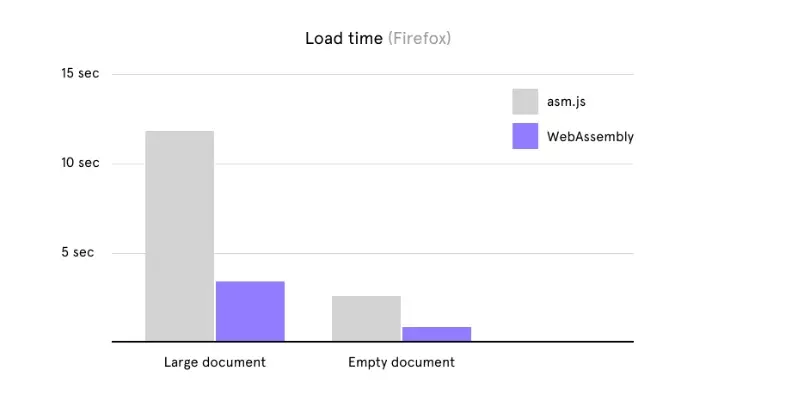
\includegraphics[width=10cm]{figma_perf.png}

    \end{center}

    \begin{center}
        3$\times$ faster load times
    \end{center}
\end{frame}

\begin{frame}
    \frametitle{Performance of Web Assembly — Fastq.bio}
    \begin{center}
        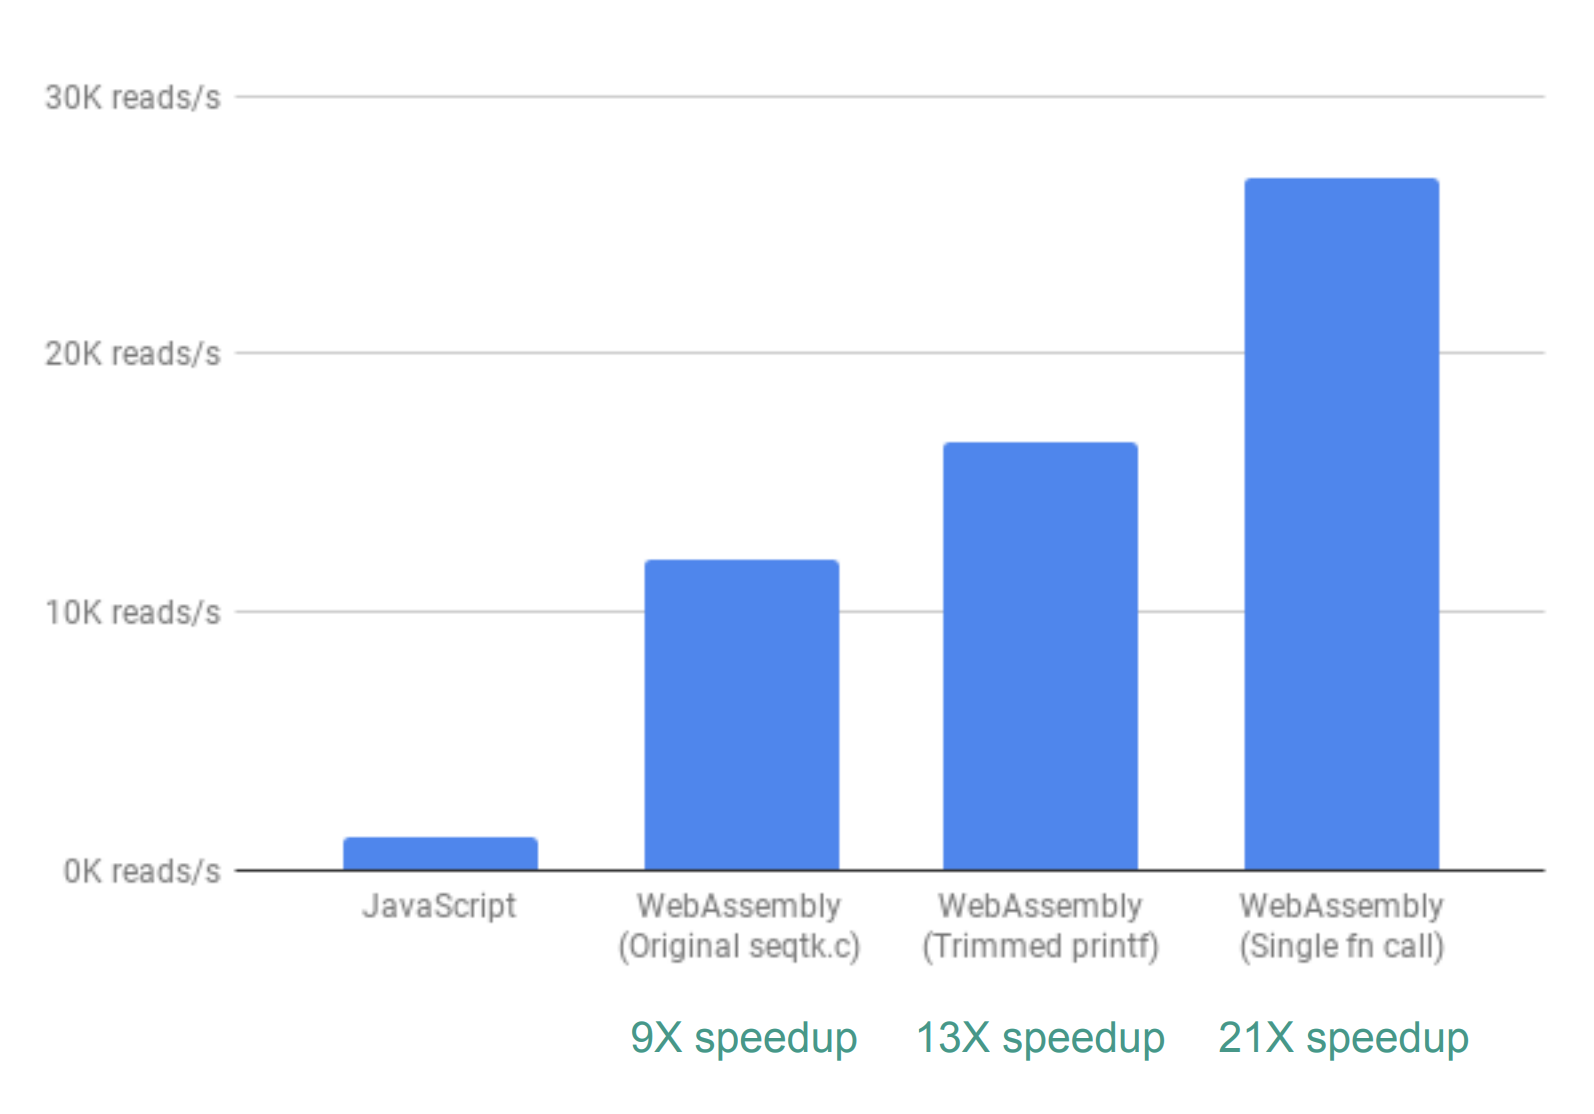
\includegraphics[width=10cm]{fastq.png}

    \end{center}
\end{frame}

\begin{frame}
    \frametitle{Performance of Web Assembly — Compared to native}

    {\small
        \begin{table}[H]
            \centering
            \vspace*{6pt}
            \label{native}
            \begin{tabular}{cccc}\hline\hline
                Benchmark & Field                   & Native time(s) & Google Chrome time(s) \\ \hline
                bzip2     & Compression             & 370            & 864                   \\
                mcf       & Combinatorial           & 221            & 180                   \\
                milc      & Chromodynamics          & 375            & 369                   \\
                namd      & Molecular Dynamics      & 271            & 369                   \\
                gobmk     & Artificial Intelligence & 352            & 537
            \end{tabular}
        \end{table}
    }
\end{frame}

\begin{frame}
    \frametitle{How does it compare?}
\end{frame}

\begin{frame}
    \vfill
    \centering
    \begin{beamercolorbox}[sep=8pt,center,shadow=true,rounded=true]{title}
        \usebeamerfont{title} My Solution\par%
    \end{beamercolorbox}
    \vfill
\end{frame}

\begin{frame}
    \frametitle{Brightness}
    \begin{center}
        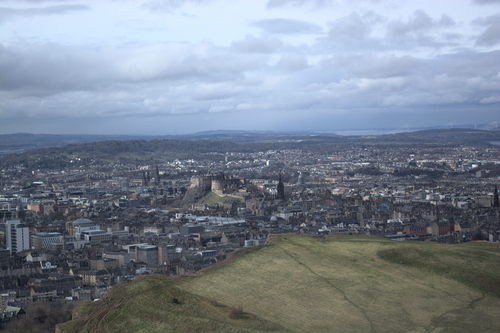
\includegraphics[width=0.48\textwidth]{default.png}
        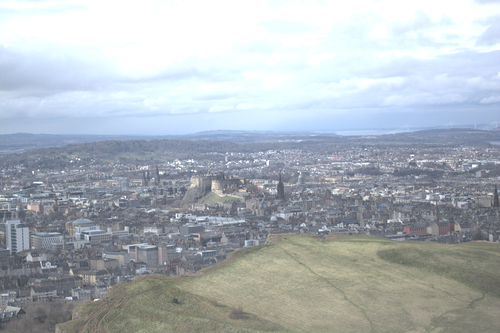
\includegraphics[width=0.48\textwidth]{bright.png}
    \end{center}

\end{frame}

\begin{frame}
    \frametitle{Contrast}
    \begin{center}
        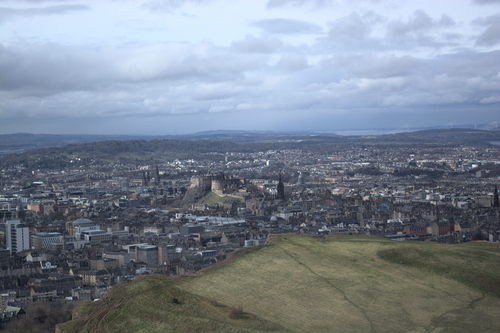
\includegraphics[width=0.48\textwidth]{default.png}
        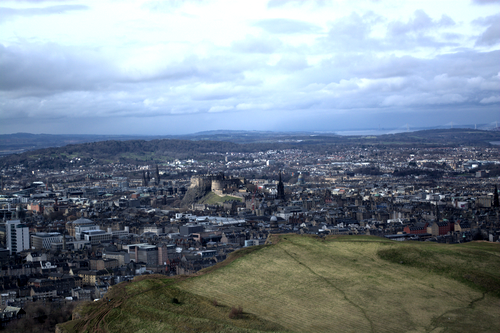
\includegraphics[width=0.48\textwidth]{contrast.png}
    \end{center}

\end{frame}

\begin{frame}
    \frametitle{Gaussian Blur}
    \begin{center}
        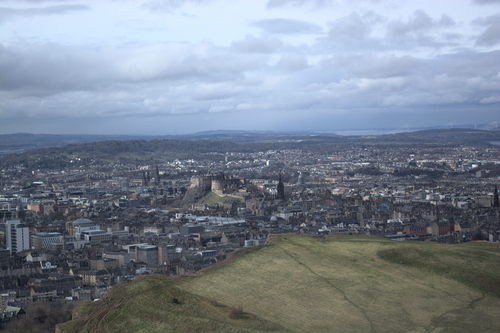
\includegraphics[width=0.48\textwidth]{default.png}
        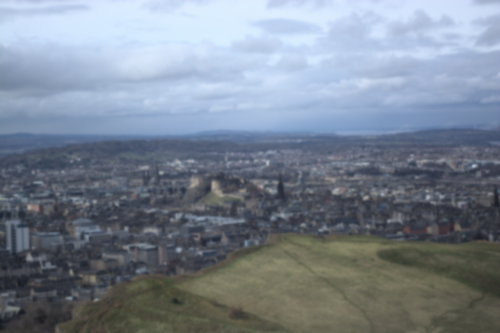
\includegraphics[width=0.48\textwidth]{blur.png}
    \end{center}

\end{frame}

\begin{frame}
    \frametitle{JPEG — YCbCr Conversion}
    \begin{center}
        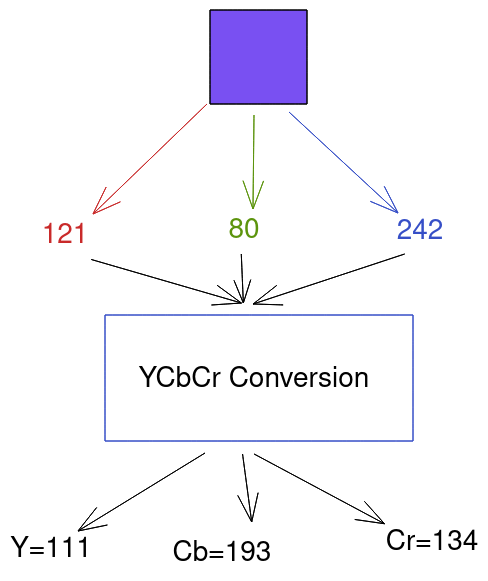
\includegraphics[width=0.48\textwidth]{ycbcr.png}
    \end{center}
\end{frame}

\begin{frame}
    \frametitle{JPEG — Downsampling}
    \begin{center}
        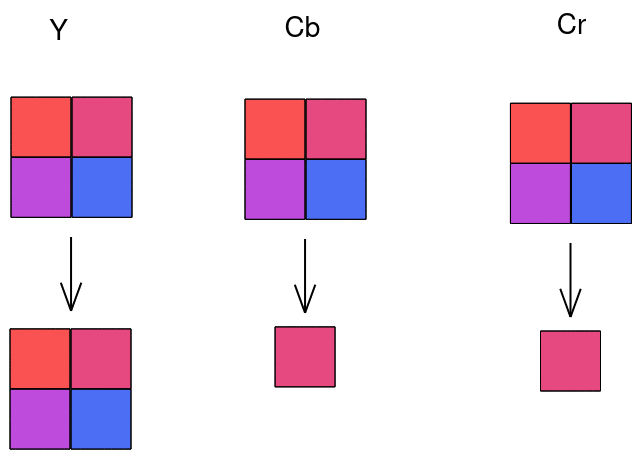
\includegraphics[width=0.8\textwidth]{downsampling.png}
    \end{center}
\end{frame}

\begin{frame}
    \vfill
    \centering
    \begin{beamercolorbox}[sep=8pt,center,shadow=true,rounded=true]{title}
        \usebeamerfont{title} Results\par%
    \end{beamercolorbox}
    \vfill
\end{frame}

\begin{frame}
    \frametitle{Complex Algorithms}
    \begin{figure}[H]
        \centering
        \begin{tikzpicture}
            \begin{axis}[
                    symbolic x coords={JavaScript, Web Assembly},
                    xtick=data,
                    bar width = 20,
                    enlarge x limits = 0.5,
                    ybar,
                    ylabel = Time(Seconds),
                    ymin=0,
                    nodes near coords,
                    axis x line*=bottom,
                    axis y line*=left,
                    width=200,
                    legend style={at={(0.5,-0.15)},
                            anchor=north,legend columns=-1}		]
                \addplot coordinates {
                        (JavaScript,   2.48)
                        (Web Assembly,  1.60)
                    };
                \addplot coordinates {
                        (JavaScript,   12)
                        (Web Assembly,  1.14)
                    };
                \legend{JPEG Encoding,Gaussian Blur}
            \end{axis}
        \end{tikzpicture}
    \end{figure}
\end{frame}

\begin{frame}
    \frametitle{Simple Algorithms}

    \begin{figure}[H]
        \centering
        \begin{tikzpicture}
            \begin{axis}[
                    symbolic x coords={JavaScript, Web Assembly},
                    xtick=data,
                    bar width = 20,
                    enlarge x limits = 0.5,
                    ybar,
                    ylabel = Time(Milliseconds),
                    ymin=0,
                    nodes near coords,
                    axis x line*=bottom,
                    axis y line*=left,
                    width=200,
                    legend style={at={(0.5,-0.15)},
                            anchor=north,legend columns=-1}		]
                \addplot coordinates {
                        (JavaScript,   102)
                        (Web Assembly,  77)
                    };
                \addplot coordinates {
                        (JavaScript,   103)
                        (Web Assembly,  278)
                    };
                \legend{Brightness, Contrast}
            \end{axis}
        \end{tikzpicture}
    \end{figure}

\end{frame}

\begin{frame}
    \frametitle{Time for the full process}
    \begin{figure}[H]
        \centering
        \begin{tikzpicture}
            \begin{axis}[
                    symbolic x coords={JavaScript, Web Assembly, imagemagick},
                    xtick=data,
                    bar width = 20,
                    enlarge x limits = 0.2,
                    ybar,
                    ylabel = Time(Seconds),
                    ymin=0,
                    nodes near coords,
                    axis x line*=bottom,
                    axis y line*=left,
                    width=300,
                    height=200		]
                \addplot coordinates {
                        (JavaScript,  3.17)
                        (Web Assembly,  2.79)
                        (imagemagick,  0.37)
                    };
            \end{axis}
        \end{tikzpicture}
    \end{figure}
\end{frame}

\begin{frame}
    \frametitle{Memory consumption of the full process}
    \begin{figure}[H]
        \centering
        \begin{tikzpicture}
            \begin{axis}[
                    symbolic x coords={JavaScript, Web Assembly, imagemagick},
                    xtick=data,
                    bar width = 20,
                    enlarge x limits = 0.2,
                    ybar,
                    ylabel = Memory (Megabytes),
                    ymin=0,
                    nodes near coords,
                    axis x line*=bottom,
                    axis y line*=left,
                    width=300,
                    height=200		]
                \addplot coordinates {
                        (JavaScript,  61.4)
                        (Web Assembly,  28.8)
                        (imagemagick,  10.6)
                    };
            \end{axis}
        \end{tikzpicture}
    \end{figure}
\end{frame}




\begin{frame}
    \frametitle{Evaluation}
    \begin{itemize}
        \item[\Checkmark] Faster
        \item[\Checkmark] Lower memory consumption
        \item[\Checkmark] Static types
        \item[\XSolidBrush] Static types
        \item[\XSolidBrush] Slower than native
        \item[\XSolidBrush] Need to use multiple languages
        \item[\XSolidBrush] Libraries have had less development
    \end{itemize}
\end{frame}

\begin{frame}
    \frametitle{Further Work}
    \begin{itemize}
        \item WebGPU
        \item Different methods
        \item Different languages
    \end{itemize}
\end{frame}

\end{document}